\section{Google Analytics Crash Reports to Email Guide} \label{ChapCrashReport}
\textit{This is a step for step guide for the setting up crash reports from Google analytics to email, for the google analytics group of 2016.}

\begin{enumerate}
	\item The first thing to do is to go to the google analytics website at http://www.google.com/analytics/ 
	\item Then log in to the google account using the google account information provided.
	\item The page should then look like shown below on figure \ref{MainPage}.
		\begin{figure}[H]
			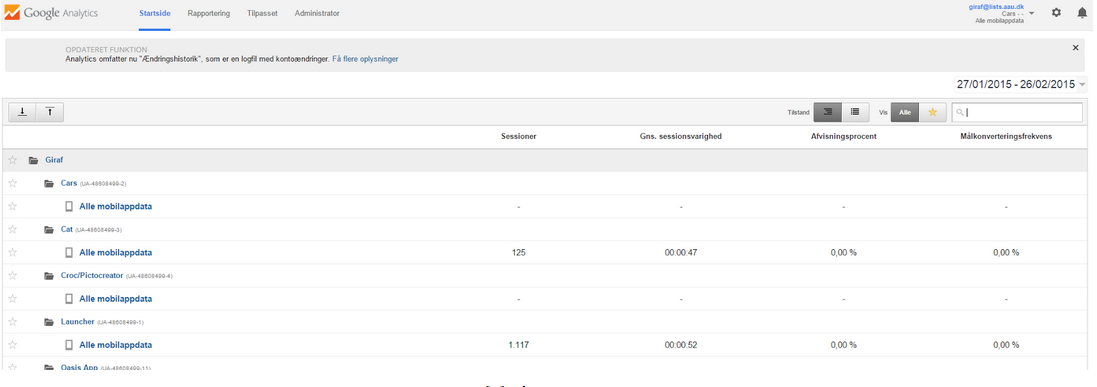
\includegraphics[width=0.8 \textwidth]{pictures/MainPage.png}
			\caption{Main page when logged in to Google analytics}
			\label{MainPage}
		\end{figure}
	\item Select the app you want to have a crash report from by pressing “Alle mobile appdata” Right below the app.
	\item This should then lead you to a page like on figure \ref{Appoversigt} the one below.
		\begin{figure}[H]
			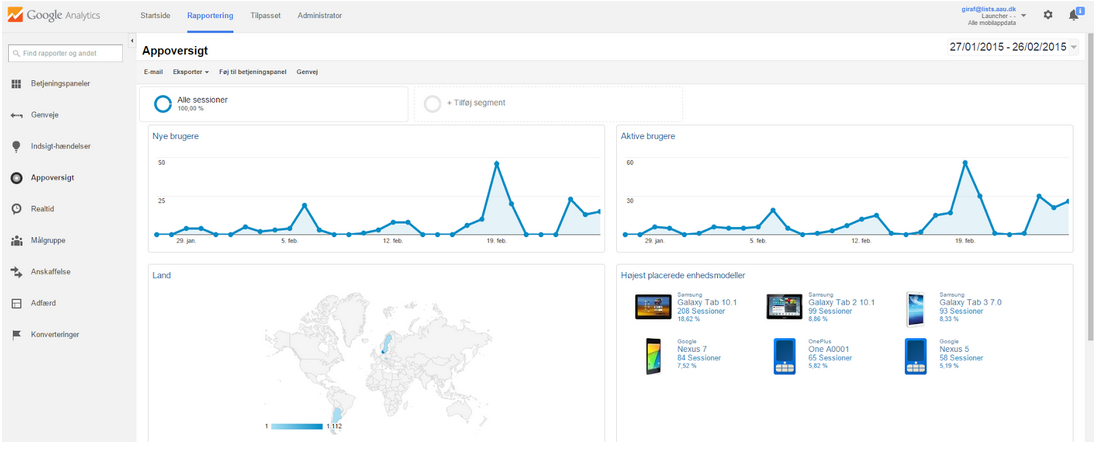
\includegraphics[width=0.8 \textwidth]{pictures/Appoversigt.png}
			\caption{App overview page}
			\label{Appoversigt}
		\end{figure}
	\item At the left most sidebar, press on “Adfærd”/”Behavior” and select “Nedbrud og Undtagelser”/”Crashes and Exceptions” in the dropdown menu.
	\item The Page should then look like shown below on figure \ref{CrashesAndExceptions}.
		\begin{figure}[H]
			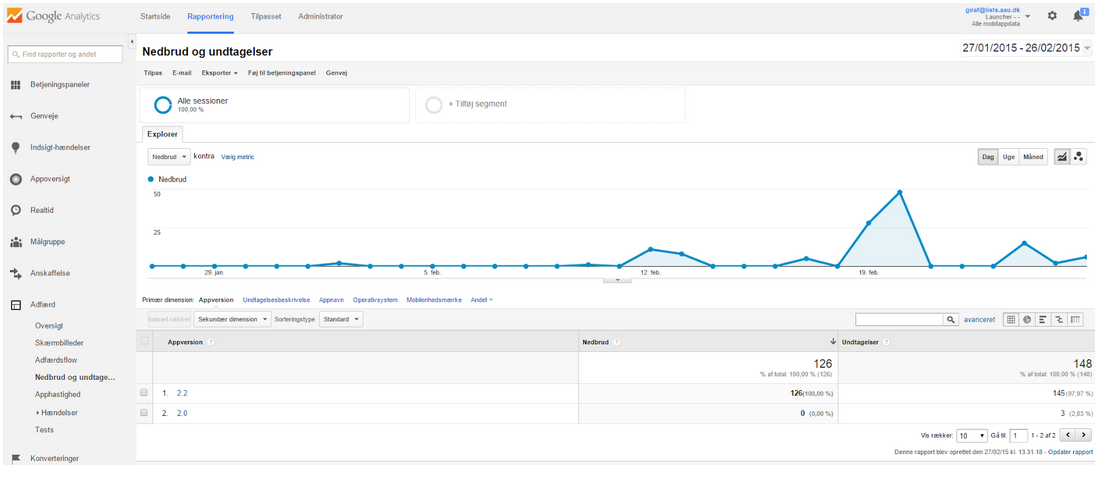
\includegraphics[width=0.8 \textwidth]{pictures/CrashesAndExceptions.png}
			\caption{Crashes and Exceptions page}
			\label{CrashesAndExceptions}
		\end{figure}	
	\item At the bottom of the page click on the newest version of the app.
	\item The page should then show all the crashes at the bottom of the screen.
	\item After this go to the top right of the page and click on the date interval.
	\item This should open a window like the one shown below on figure \ref{Calender}.
		\begin{figure}[H]
			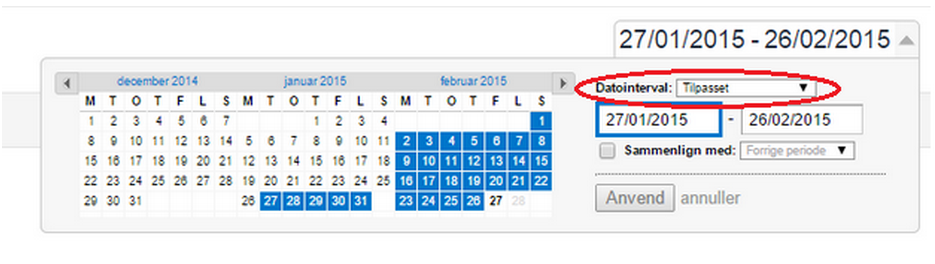
\includegraphics[width=0.8 \textwidth]{pictures/Calender.png}
			\caption{Calender window}
			\label{Calender}
		\end{figure}
	\item In the window select the time interval that you want the crash report to be sent from in the highlighted dropdown menu.
	\item Press “Anvend”/”Apply” to close the window.
	\item In one of the top menus there is a button named “Email”, press it.
		\begin{figure}[H]
			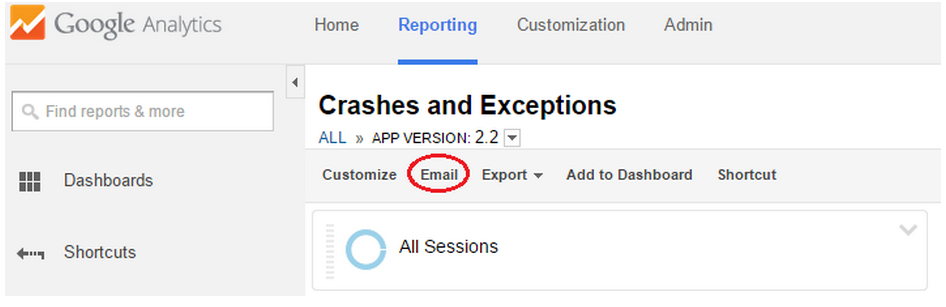
\includegraphics[width=0.8 \textwidth]{pictures/Email.png}
			\caption{Email button}
			\label{Email}
		\end{figure}
	\item In the window that opens select whom to send the mail to, what format the crash report should be in, and when the email should be send.
		\begin{figure}[H]
			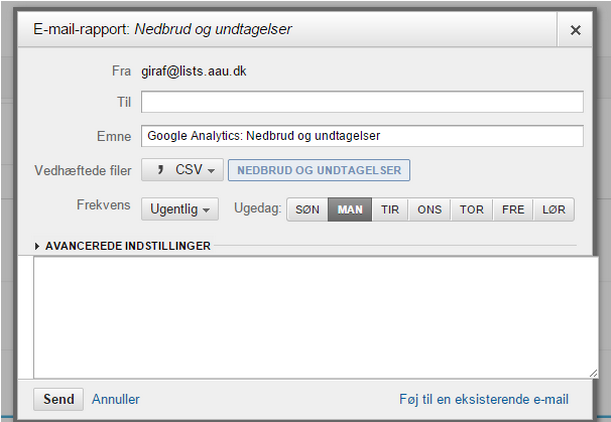
\includegraphics[width=0.8 \textwidth]{pictures/Maillist.png}
			\caption{Mail report window}
			\label{Maillist}
		\end{figure}
\end{enumerate}
	